\documentclass[border=5pt]{standalone}
\usepackage{tikz}
\usetikzlibrary{arrows.meta, positioning, decorations.pathreplacing, calc}
\usepackage{xcolor}

\definecolor{Garnet}{HTML}{73000A}
\definecolor{NinetyBlack}{HTML}{363636}
\definecolor{SeventyBlack}{HTML}{5C5C5C}
\definecolor{FiftyBlack}{HTML}{A2A2A2}
\definecolor{ThirtyBlack}{HTML}{C7C7C7}
\definecolor{TenBlack}{HTML}{ECECEC}
\definecolor{Atlantic}{HTML}{466A9F}
\definecolor{Horseshoe}{HTML}{65780B}
\definecolor{Sandstorm}{HTML}{FFF2E3}

\tikzset{every node/.append style={rounded corners=0pt}}

\begin{document}
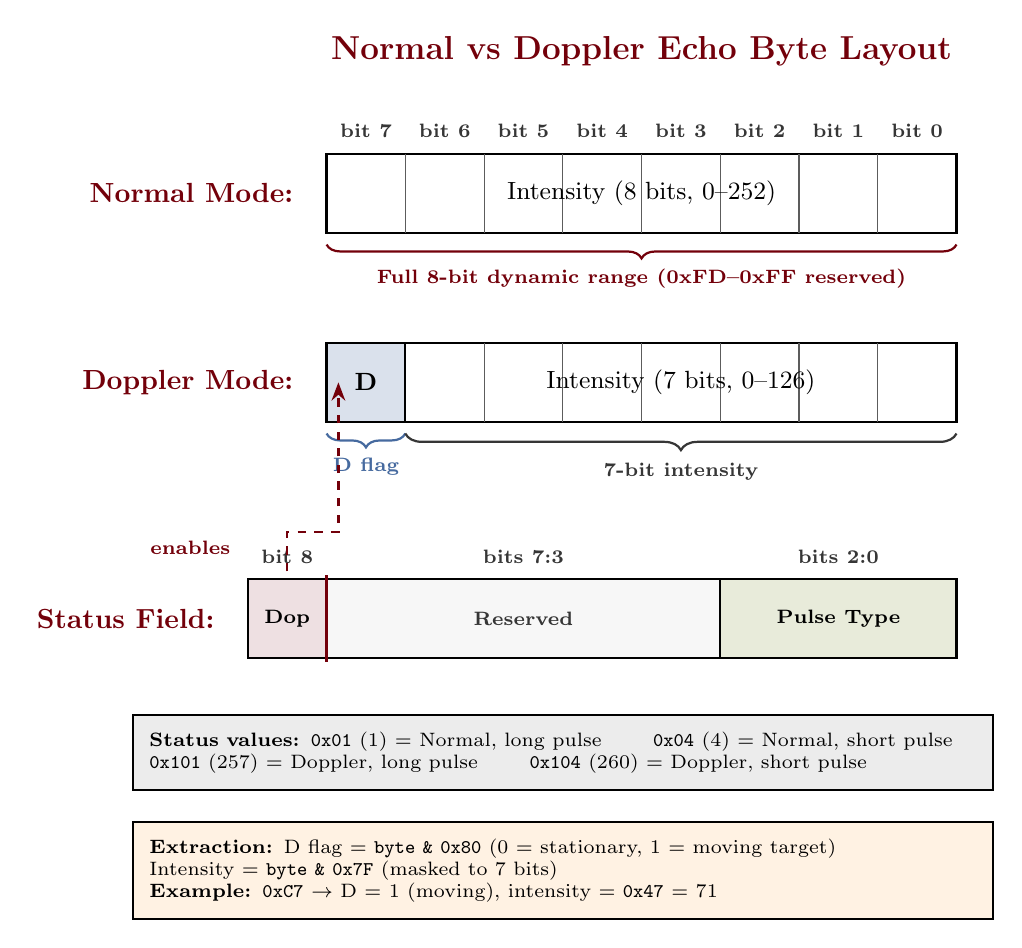
\begin{tikzpicture}[
    lbl/.style={font=\small\bfseries, color=NinetyBlack},
    annot/.style={font=\scriptsize, color=SeventyBlack},
]

% ── Title ──
\node[font=\bfseries\large, color=Garnet] at (4, 11.0) {Normal vs Doppler Echo Byte Layout};

% ── Bit position labels ──
\foreach \i/\v in {0/7, 1/6, 2/5, 3/4, 4/3, 5/2, 6/1, 7/0} {
    \node[font=\scriptsize\bfseries, color=NinetyBlack] at (0.5 + \i*1.0, 10.0) {bit \v};
}

% ── Normal Mode box ──
\node[font=\bfseries\color{Garnet}, anchor=east] at (-0.3, 9.2) {Normal Mode:};
\draw[thick] (0, 8.7) rectangle (8, 9.7);
\foreach \x in {1,...,7} {
    \draw[thin, SeventyBlack] (\x, 8.7) -- (\x, 9.7);
}
\node[font=\small] at (4, 9.2) {Intensity (8 bits, 0--252)};

% Brace below normal mode
\draw[decorate, decoration={brace, amplitude=5pt, mirror}, thick, Garnet]
    (0, 8.55) -- (8, 8.55) node[midway, below=5pt, font=\scriptsize\bfseries, color=Garnet]
    {Full 8-bit dynamic range (0xFD--0xFF reserved)};

% ── Doppler Mode box ──
\node[font=\bfseries\color{Garnet}, anchor=east] at (-0.3, 6.8) {Doppler Mode:};
\draw[thick] (0, 6.3) rectangle (8, 7.3);
% D flag bit (bit 7) — filled
\draw[thick, fill=Atlantic!20] (0, 6.3) rectangle (1, 7.3);
\node[font=\small\bfseries] at (0.5, 6.8) {D};
% Thick divider between D flag and intensity
\draw[thick] (1, 6.3) -- (1, 7.3);
% 6 thin dividers inside the 7-bit intensity region (x=2..7)
\foreach \x in {2,...,7} {
    \draw[thin, SeventyBlack] (\x, 6.3) -- (\x, 7.3);
}
\node[font=\small] at (4.5, 6.8) {Intensity (7 bits, 0--126)};

% Braces below Doppler mode — staggered vertically
\draw[decorate, decoration={brace, amplitude=5pt, mirror}, thick, Atlantic]
    (0, 6.15) -- (1, 6.15) node[midway, below=5pt, font=\scriptsize\bfseries, color=Atlantic] {D flag};
\draw[decorate, decoration={brace, amplitude=6pt, mirror}, thick, NinetyBlack]
    (1, 6.15) -- (8, 6.15) node[midway, below=7pt, font=\scriptsize\bfseries, color=NinetyBlack] {7-bit intensity};

% ── Status Field (9 bits: bit 8 extends left of the 8-bit column grid) ──
\node[font=\bfseries\color{Garnet}, anchor=east] at (-1.3, 3.8) {Status Field:};

% Bit 8 (Doppler active) — offset left, outside the 8-bit grid
\draw[thick, fill=Garnet!12] (-1, 3.3) rectangle (0, 4.3);
\node[font=\scriptsize\bfseries] at (-0.5, 3.8) {Dop};
\node[font=\scriptsize\bfseries, color=NinetyBlack, above=2pt] at (-0.5, 4.3) {bit 8};

% Bits 7:3 (Reserved) — aligned with byte grid
\draw[thick, fill=ThirtyBlack!15] (0, 3.3) rectangle (5, 4.3);
\node[font=\scriptsize\bfseries, color=NinetyBlack] at (2.5, 3.8) {Reserved};
\node[font=\scriptsize\bfseries, color=NinetyBlack, above=2pt] at (2.5, 4.3) {bits 7:3};

% Bits 2:0 (Pulse Type) — aligned with byte grid
\draw[thick, fill=Horseshoe!15] (5, 3.3) rectangle (8, 4.3);
\node[font=\scriptsize\bfseries] at (6.5, 3.8) {Pulse Type};
\node[font=\scriptsize\bfseries, color=NinetyBlack, above=2pt] at (6.5, 4.3) {bits 2:0};

% Double-line boundary between bit 8 and bits 7:0
\draw[very thick, Garnet] (0, 3.25) -- (0, 4.35);

% ── Visual link: Status Dop flag → Doppler D flag ──
% Arrow: up from Dop, jog right at y=4.9 (well below brace labels), then up into D cell
\draw[-{Stealth}, thick, Garnet, dashed]
    (-0.5, 4.4) -- (-0.5, 4.9) -- (0.15, 4.9) -- (0.15, 6.8);
% Label on the horizontal segment
\node[font=\scriptsize\bfseries, color=Garnet, anchor=east] at (-1.1, 4.7) {enables};

% ── Status value examples ──
\node[draw, thick, fill=TenBlack, text width=10.5cm, align=left, font=\scriptsize, inner sep=6pt] at (3.0, 2.1) {
\textbf{Status values:}
\texttt{0x01} (1) = Normal, long pulse \qquad
\texttt{0x04} (4) = Normal, short pulse \\
\texttt{0x101} (257) = Doppler, long pulse \qquad
\texttt{0x104} (260) = Doppler, short pulse
};

% ── Extraction formulas ──
\node[draw, thick, fill=Sandstorm, text width=10.5cm, align=left, font=\scriptsize, inner sep=6pt] at (3.0, 0.6) {
\textbf{Extraction:}
D flag = \texttt{byte \& 0x80} (0 = stationary, 1 = moving target) \\
Intensity = \texttt{byte \& 0x7F} (masked to 7 bits) \\
\textbf{Example:} \texttt{0xC7} $\rightarrow$ D = 1 (moving), intensity = \texttt{0x47} = 71
};

\end{tikzpicture}
\end{document}
